
\documentclass[conference]{IEEEtran}
\IEEEoverridecommandlockouts
% The preceding line is only needed to identify funding in the first footnote. If that is unneeded, please comment it out.
%Template version as of 6/27/2024

\usepackage{cite}
\usepackage{amsmath,amssymb,amsfonts}
\usepackage{algorithmic}
\usepackage{graphicx}
\usepackage{textcomp}
\usepackage{xcolor}
\usepackage{siunitx}

\def\BibTeX{{\rm B\kern-.05em{\sc i\kern-.025em b}\kern-.08em
    T\kern-.1667em\lower.7ex\hbox{E}\kern-.125emX}}
\begin{document}

\title{A Compact, Low-cost Sensor Suite  for Laboratory Experiments
}

\author{}
\maketitle

\begin{abstract}
This demo describes a new concept in the development of Physics Laboratory experiments 
 following  the Do-It-Yourself (DYI) philosophy, showing to students that sophisticated experiments may be conducted using off-the-self electronic equipment.
It also provides with an University teaching staff an increased flexibility in preparing and conducting experiments. 
This does not aim to replace traditional laboratory experiments which resort to more sophisticated and dedicated equipment,
but instead to complement such experiments with more simplified experiments that may be setup on an as needed basis.
The authors will present at the exhibition one or two live experiments, and the participants will be invited to play 
and take measurements of physical quantities with great precision.

\end{abstract}

\begin{IEEEkeywords}
Physics, Laboratory Experiments, Remote Control, Online Data.
\end{IEEEkeywords}

\section{Introduction}
% Framework
The availability of widespread, cheap, and relatively powerful electronic devices provides for unique and exciting opportunities for developing flexible, ``off-the-shelf'' laboratory experiments where a suite of diagnostics can be deployed to monitor and instrument generic devices under study.

Besides the ubiquitous, low-level diagnostics available in the laboratory environment (such as multi-meters, or even generic, low cost oscilloscopes), it is now possible to develop very cheap and reliable diagnostic devices to measure quantities such as  
Temperatures, Pressure, Force, Magnetic field, Electric ($V$, $I$ and $R$), Movement, Sound, etc (e.g. a kit box with more than 50 sensors can be bought online for $<$ 10€).

In addition to this we now have access to cheap and rugged "embedded computer” solutions, chiefly the Raspberry-Pi, Arduino\cite{b2} and compatible suites.
These allow for a fully customized, dedicated online connected computer capable of handling very reasonable acquisition rates (around 10kHz) 
and delivering the resulting data in electronic form. 
The experimental data can be upload to open databases and the students can easily retrieve 
 directly to standard generic (e.g. Excel), or more advanced data processing tools
 (MATLAB, Python, etc.)

The main objectives were to develop an open ecosystem with a flexible, low-cost suite of diagnostics with an ``uncomplicated'' interface; ii) capitalize on the significant developments/cost reductions that have taken place in the last decades regarding micro-controllers/microcomputers, and iii)

\section{Architecture}
The hardware backbone for this platform consists in a combination of a Raspberry-Pi (RPi) board computer and an Arduino compatible board. 
The Rpi will host all the developing  apps, communications infrastructure, database server, online servers (Apache, Grafana). 
 A cabled Ethernet connection is preferable, but not  required, since the RPi is able to use an Wifi connection, 
 for example using the "Hop-Spot" function on the instructor’s smartphone, also shared to the student’s phones or mobile PCs.

 The experiment sensor's will be connected to an Arduino board, or compatible.
 Most promising and cost effective units presently are the ESP32 micro-controller based devices, in particular the M5Stick-CP2,
 that are fully wireless, since include a battery and connect directly to Wifi.
 %(An example is shown in `Fig.~\ref{figM5}'')

 Two different architectures are envisaged, one Unitary is used by the instructor during regular classes, 
 and one Multiple (``Fig.~\ref{figMultiple}''),
 where a complete hardware kit is lend to groups/individuals. 
 In both configurations all experimental data is stored in Cloud-based Time Series Database\cite{b3} (TSDB).
 
\begin{figure}[htbp]
\centerline{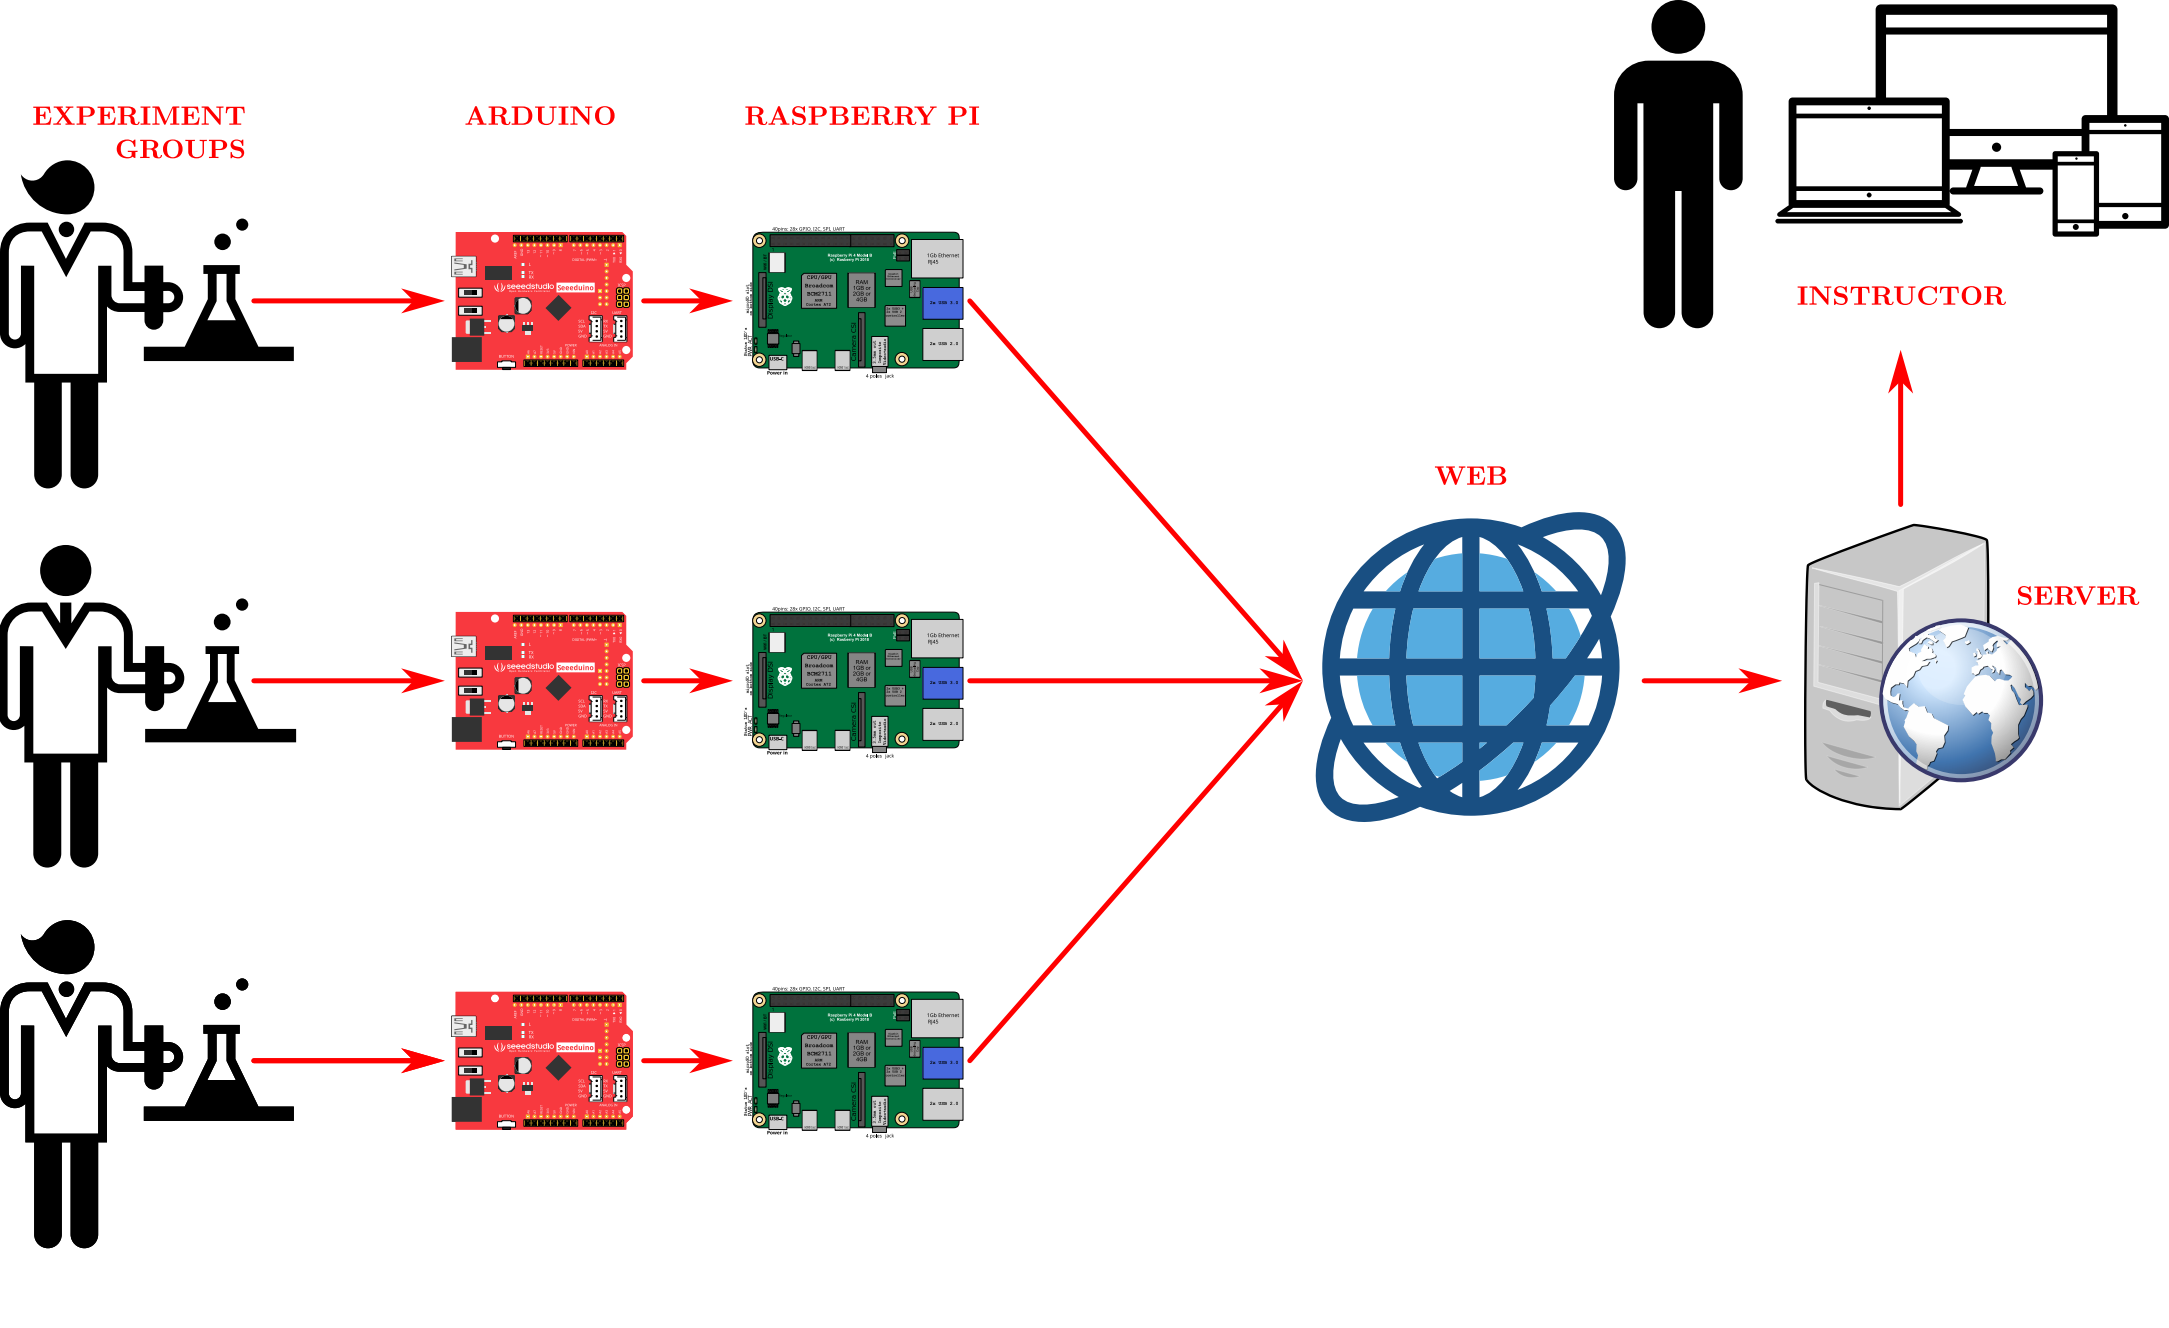
\includegraphics[width=.6\columnwidth]{Multiple.png}}
\caption{Several groups perform the experiment in class and upload the results to a server.}
\label{figMultiple}
\end{figure}

The two computing boards plus all the hardware necessary to assemble a specific Experiment, will placed in stackable briefcases.
%used to transport each individual set of experiments.
Each briefcase size is “1 Storage Unit” (1SU), allowing easy and flexible transportation of up to 4-5 sets of experiments with a small trolley.


\section{Applications}
The equipment is to be applied to a very wide range of experiments, ranging from under-graduate courses laboratory experiments (fundamental physics), 
to more advanced experiments in master courses. 
But most of all, the equipment is to have robust and well-maintained documentation, 
following the best “Open” software/hardware practices, encouraging users to come up with novel experiments.

A live library of experiments, with a description of the selected instrumentation, and the associated tailored code will be maintained and made available in a seamless fashion. 
This means for example providing dedicated ISO’s that only require flashing on the Raspberry/Arduino SD cards, after which the diagnostic setup is ready for deployment,
or a more sophisticated option of providing a library of configurations of the chip to be loaded on a case-by-case basis.

Each experiment would have an associated laboratory guide, either in PDF, or wiki form (or both) and one or more Jupyter\cite{b4} Notebooks ready to be used by students. 

A dedicated platform for exchange of information/code/documentation/etc. was developed and hosted on a public Github\cite{gh} repository. 
At later stages of the project, after successful proof-of-concept deployments of the sensor suite, more experiment will be added.


\section{Pilot Experiments}
A demo prototype was assembled and was already used in a initial set of Laboratory demonstrations. 
All demos were concluded at  undergraduate engineering IST (See ``Tab.~\ref{tab1}''), in the first part of regular classes (about 30 minutes each).
The feedback from students were strongly motivating and the suggestion that groups could experiment themselves 
or even bring then home the kit was seen as very attractive.

\begin{table}[htbp]
\caption{List of Pilot Experiments}
\begin{center}
\begin{tabular}{|c|c|c|c|}
\hline
\textbf{Degree}&\textbf{Year}&\textbf{Course} &\textbf{Experiment}\\
\hline
Civil Eng. & 2nd&  Thermodynamics & Calorimetry\\
\hline
Civil Eng. & 2nd&  Thermodynamics & Stirling Engine\\
\hline
 Electric Eng.& 1rst&  Physics (Mechanics) & Maxwell Wheel\\
\hline
\end{tabular}
\label{tab1}
\end{center}
\end{table}

\subsection{Maxwell Wheel Experiment}
The Maxwell Wheel is a introductory Physics Lab project\cite{b6} where the students are 
invited to estimate the Wheel's Inertial Momentum  $I_z$,
to do so they must perform a long and time consuming measurement series of time and velocity, 
in different positions. 
The apparatus is depicted in ``Fig.~\ref{figMaxwell}''.

\begin{figure}[htbp]
    \centerline{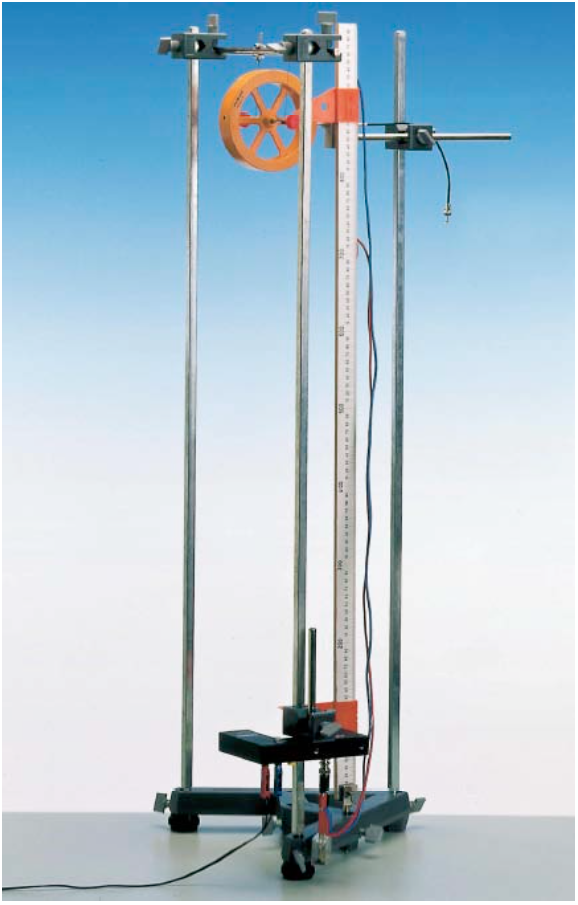
\includegraphics[width=.6\columnwidth]{maxwell.png}}
    \caption{Maxwell Wheel standart Apparatus, showing a single light barrier. Students have to change barrier for each measure point.}
\label{figMaxwell}
\end{figure}

While the wheel is  falling, the Mechanical Energy is described by :
\begin{IEEEeqnarray}{lcr}
    E_{mec}  &=&   E_{pot} +  E_{cin} +  E_{rot} \label{eq:max}\\
     &=&   m g h + \frac{1}{2} m v^2 + \frac{1}{2}  I_z w^2 \label{eq:max1}
\end{IEEEeqnarray}

Since the height, $h$, and linear velocity, $ \vec{v} = \vec{\omega} \times \vec{r}$ 
can be related to  the rotation angle, $\theta$i, ($\omega=\dot{\theta}$), the time derivative gives:
\begin{equation}
    \frac{dE_{mec}}{dt} =  -m g ( w *r)   + ( m r^2 +  I_z) w \dot{w}\label{eq:maxDer}
\end{equation}
where $r$ is the radius of the axis where the suspending wire is wounded.

Assuming Energy is kept constant, due the small attained linear speeds, we get: 
\begin{IEEEeqnarray}{lcr}
    \dot{w} &=& \gamma = \frac{m g  r}{m r^2 +  I_z} \label{eq:maxgamma}\\
     Iz &=&  m \frac{ g  r  - \gamma  r^2  }{\gamma}\label{eq:maxIz}
\end{IEEEeqnarray}

Traditionally the positions and velocity are measured  with the help of an optical barrier, that has to be moved in small steps (``Fig.~\ref{figMaxwell}''). 
The triggering device is fragile, often fails which disturb student's attention. 

Using this novel platform a small M5Stick/Arduino is attached close to the wheel's axis.
The acquisition  cycle is started for a defined interval and the wheel is left to fall. No electronic trigger is necessary, since the data in taken continuously.
The small board, while showing the value bars on  display, and sends 
 the 6 signals of the inertial measurement unit (IMU) (speed of rotation and gravity vector 3D components). The values are stored in a InfluxDB server hosted in the Rpi. 
 A Grafana server\cite{b7} allows an user friendly plotting and retrieval tool, including in mobile devices, 
 without the need to install any App other than a plain Web Browser (``Fig.~\ref{figIMU}'').

On an single experiment run, a simple Linear Fit on the angular velocity data, gives a very precise value of the angular acceleration,
that could be used to validate other sparse data point taken with the barrier.


\begin{figure}[htbp]
\centerline{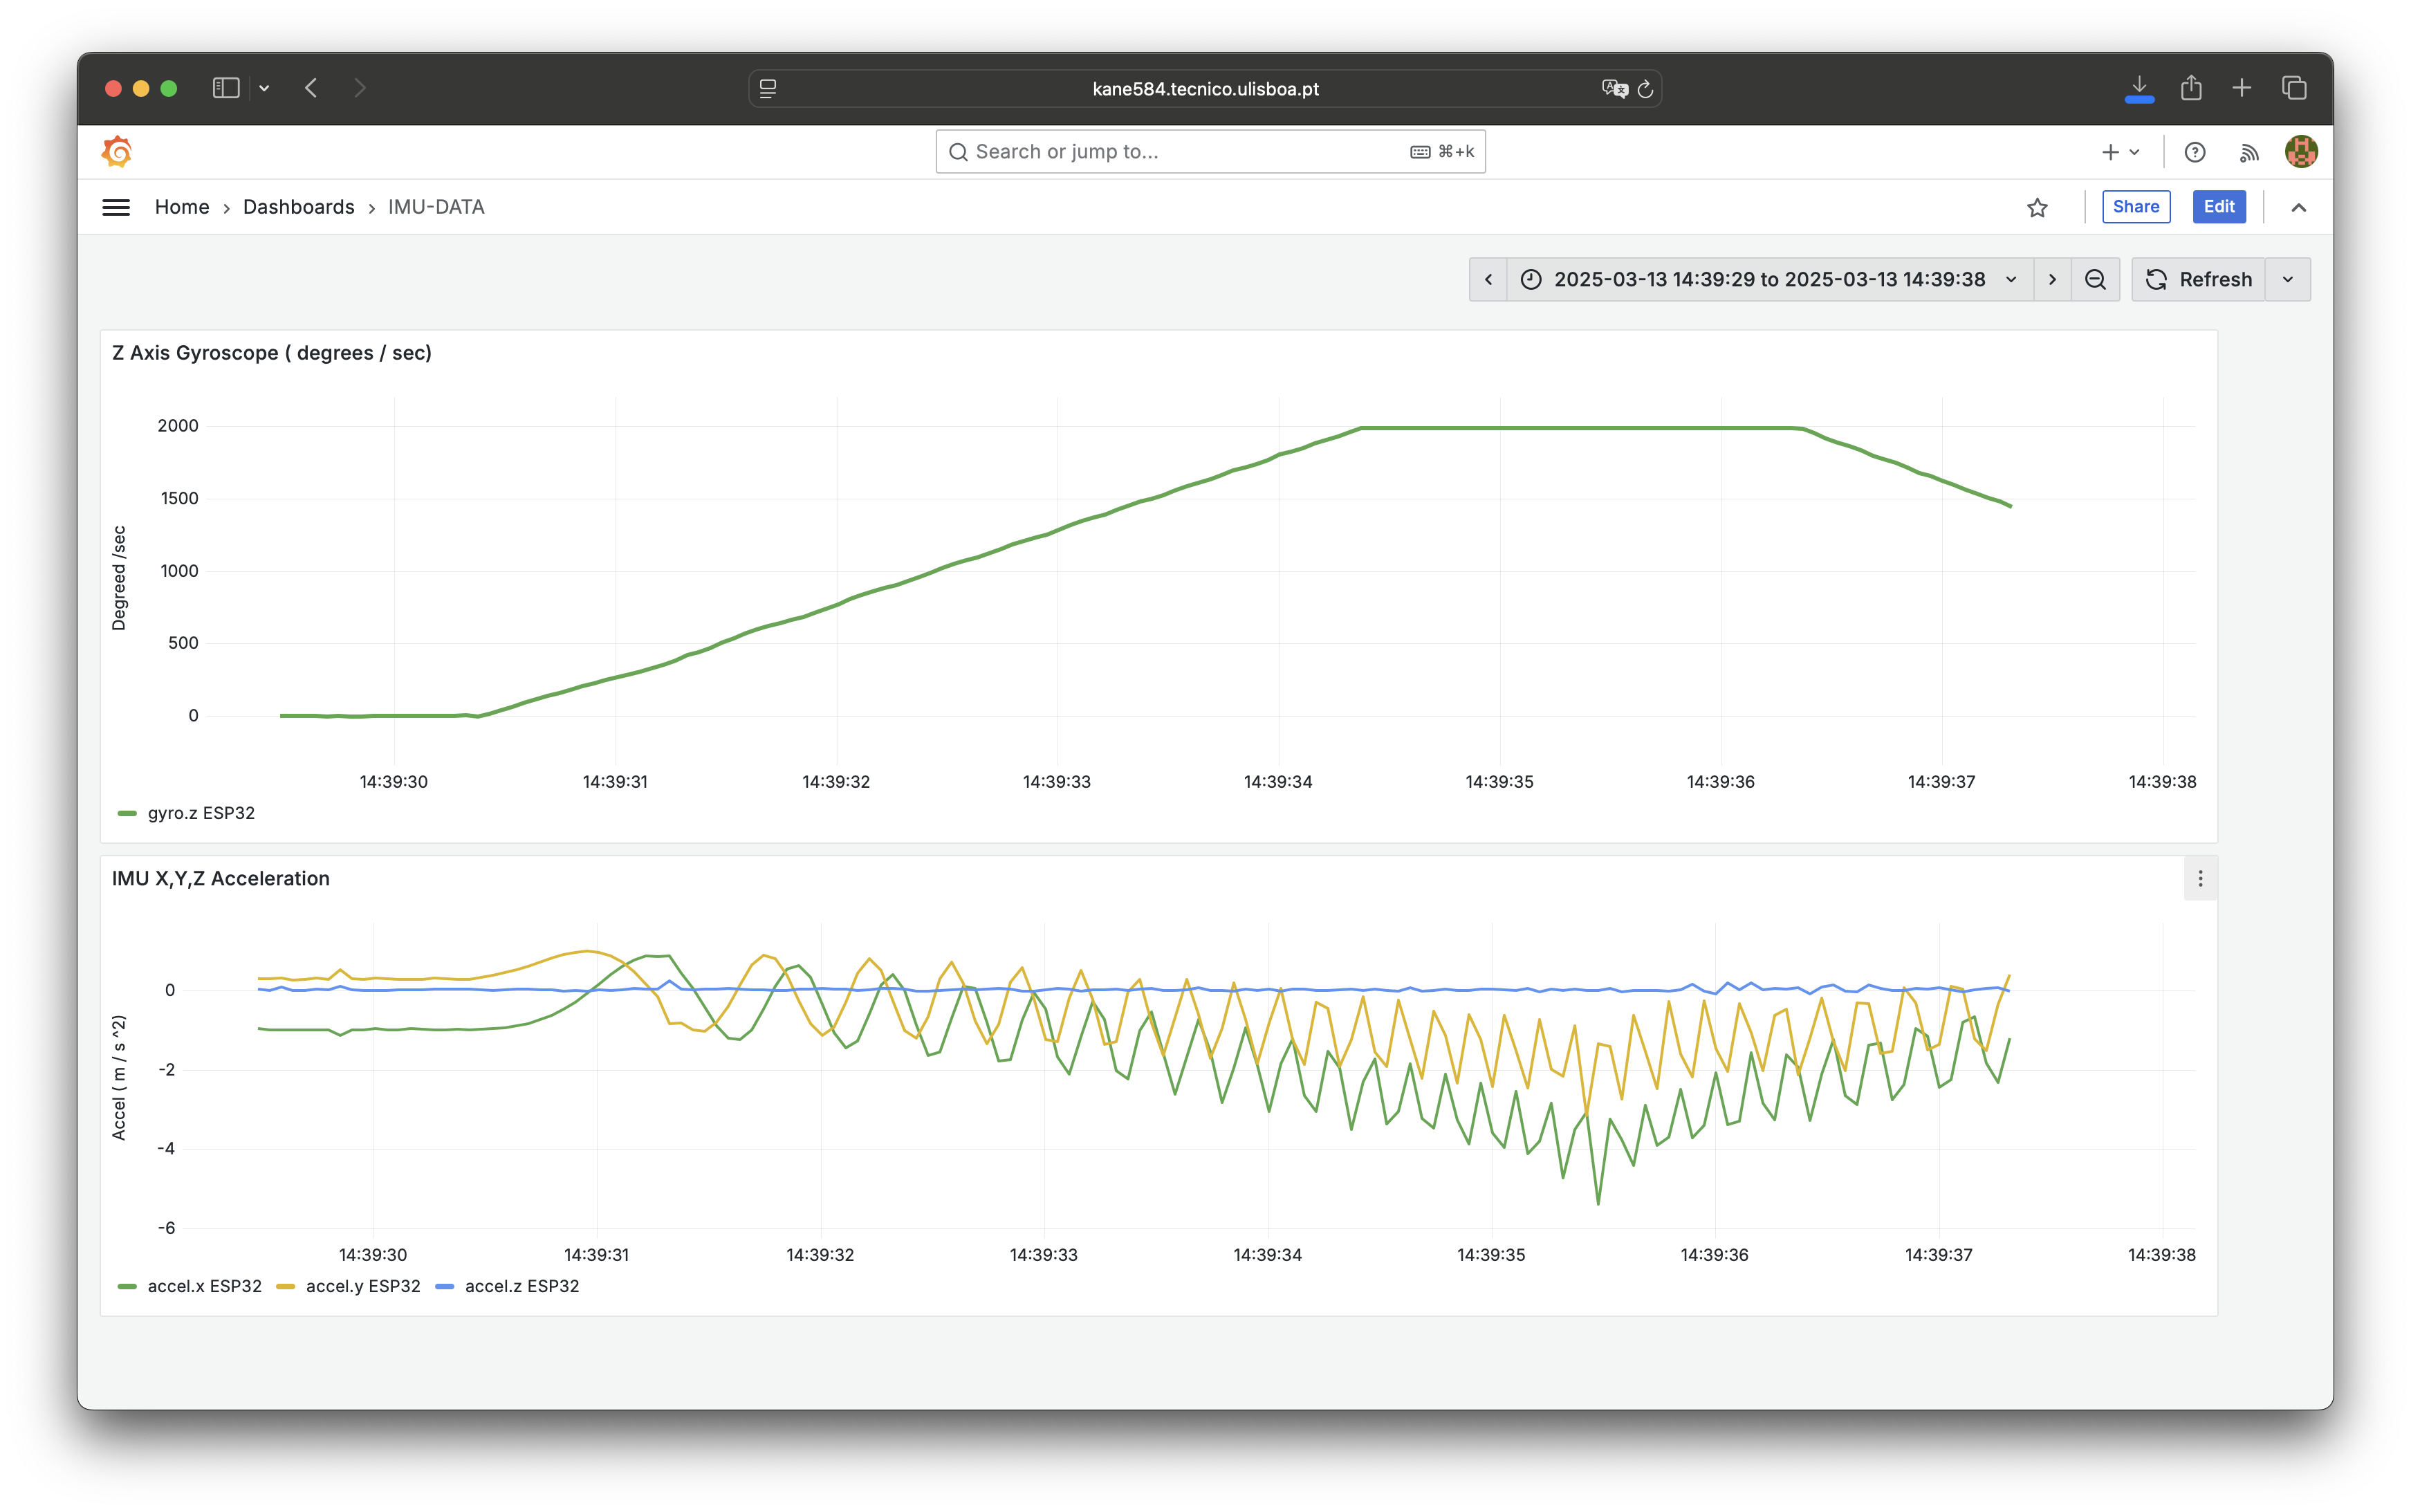
\includegraphics[width=.6\columnwidth]{IMUGrafana.png}}
\caption{Browser screeshot showing the  plotting of rotation speed (top); and angle (bottom) of the Maxwell Wheel, stored in a Grafana server}.
\label{figIMU}
\end{figure}


\subsection{Experimental results}
The data values for the Z-direction angular velocity (parallel to the Wheel's axis) were extracted using a Jupyter Notebook, as shown in ``Fig.~\ref{figAngleVel}''. 

\begin{figure}[htbp]
\centerline{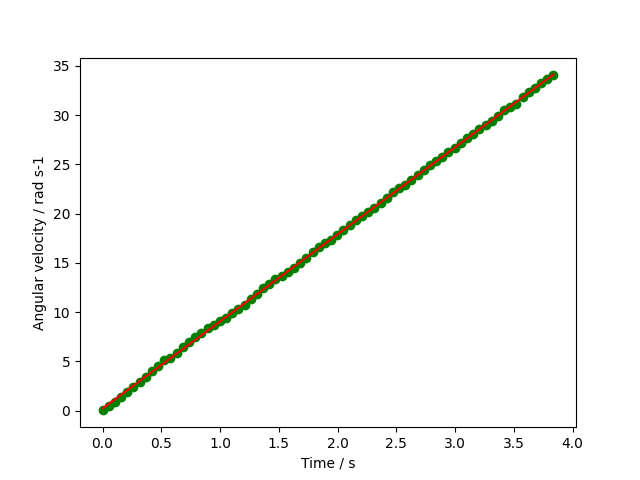
\includegraphics[width=.8\columnwidth]{AngAccel.png}}
\caption{Angular velocity plot and Linear fit.}
\label{figAngleVel}
\end{figure}

The Linear Regression on data is shown below. 
To calculate $p=95\%$ confidence interval on slope and intercept, we used a two-sided inverse Students t-distribution, with (N-2) degrees of freedom:

\begin{itemize}
    \item Slope : 8.8434 $\pm$ (rad s-2) ($\SI{0.0239}{\radian\per\second\squared}$).

    \item Intercept : 0.2022 $\pm$ $\SI{0.0531}{\radian\per\second}$.
\end{itemize}

Finally, using ``(\eqref{eq:maxIz})'', the calculated Inertial Momentum was:
\begin{equation}
     Iz  = \SI{1.43e-3}{\kg\meter\squared}
\end{equation}
with a standard error of few $\mu\SI{}{\kg\meter\squared}$, well bellow the relative precision of any instrument used in the class laboratories.
  
%\si{8.85e-12}{\coulomb\squared\per\newton\per\meter\squared}$
\section{Societal Impact in the Higher Teaching frame of reference}
This pedagogical project may potentially have a significant societal impact on the way teaching is conducted in higher education institutions, 
by bringing pinpoint capacities for simple and flexible laboratory experiments in 
teaching courses who may on a first approach not have considered the possibility for conducting experiments.
More specifically this project adheres to a certain number of key constraints:
\begin{itemize}
    \item Portability
    \item Flexibility
    \item Availability
    \item Low-cost
\end{itemize}

To conclude, and to highlight the potential for internationalization, we announce that 
this concept and prototype will be implemented at Teaching Unit @ Shangai University, Spring 2025

\begin{thebibliography}{00}
\bibitem{b1}Giovanni Organtini, ``Physics Experiments with Arduino and Smartphones,''
Springer International Publishing, January 2021, DOI: 10.1007/978-3-030-65140-4.

Physics Department, IST, February 2024.
\bibitem{b2} https://en.wikipedia.org/wiki/Arduino
\bibitem{b3} https://en.wikipedia.org/wiki/InfluxDB
\bibitem{b4} https://jupyter.org 
\bibitem{gh} https://github.com/ipfn-hpl/ard-rasp-ist
\bibitem{b6}João Mendanha, et al, ``Mechanical Energy Conservation in Maxwell Wheel, Laboratory Guide,'' (in portuguese),
\bibitem{b7} https://en.wikipedia.org/wiki/Grafana
\end{thebibliography}

\end{document}
